% CHAPTER 1
\chapter{EFFECTS OF SYNTHETIC INERTIA IMPLEMENTATION}
\label{chp:5}
The concept of synthetic inertia or virtual inertia suggest a frequency response from renewable energy systems depending on the RoCoF of the electricity grid. As explained at the end of Chapter \ref{chp:3}, a renewable energy system can provide an additional power according to the Swing Equation. In this chapter, the synthetic inertia implementation on a variable speed PMSG wind turbine is tested in P.M. Anderson 9 bus test case which is constructed in Matlab-Simulink environment. The test case is subjected to an sudden load connection in the different scenarios.
\section{P.M.Anderson 9 Bus Test Case}
\subsection{System Properties}
In order to understand frequency dynamics better, P.M. Anderson test case has been used in the study. The single line diagram of the system is given in Fig. \ref{ieee_9_bus}. The test case consists of three generators and three loads. Generators in the system are connected to 230 kV high voltage (HV) network with step-up transformers.\par
The biggest generator in the system is a hydro power plant with a power rating of 247.5 MVA. The remaining ones are steam generators. The power ratings of the generators are given in Table \ref{generatorproperties}.The loads in the system are connected directly to the HV network. The active and reactive power ratings of the loads are listed in Table \ref{loadproperties}.
\begin{table}[h]
	\centering
	\begin{tabular}{ccc}
		\hline
		\textbf{Generators} & \textbf{Power Rating (MVA)} & \textbf{Plant Type} \\ \hline
		Gen 1               & 247.5                       & Hydro				\\
		Gen 2               & 192                         & Steam               \\
		Gen 3               & 128                         & Steam               \\ \hline
	\end{tabular}
	\caption{Generator Properties of Test System}
	\label{generatorproperties}
\end{table}
\begin{figure}[h]
	\centering
	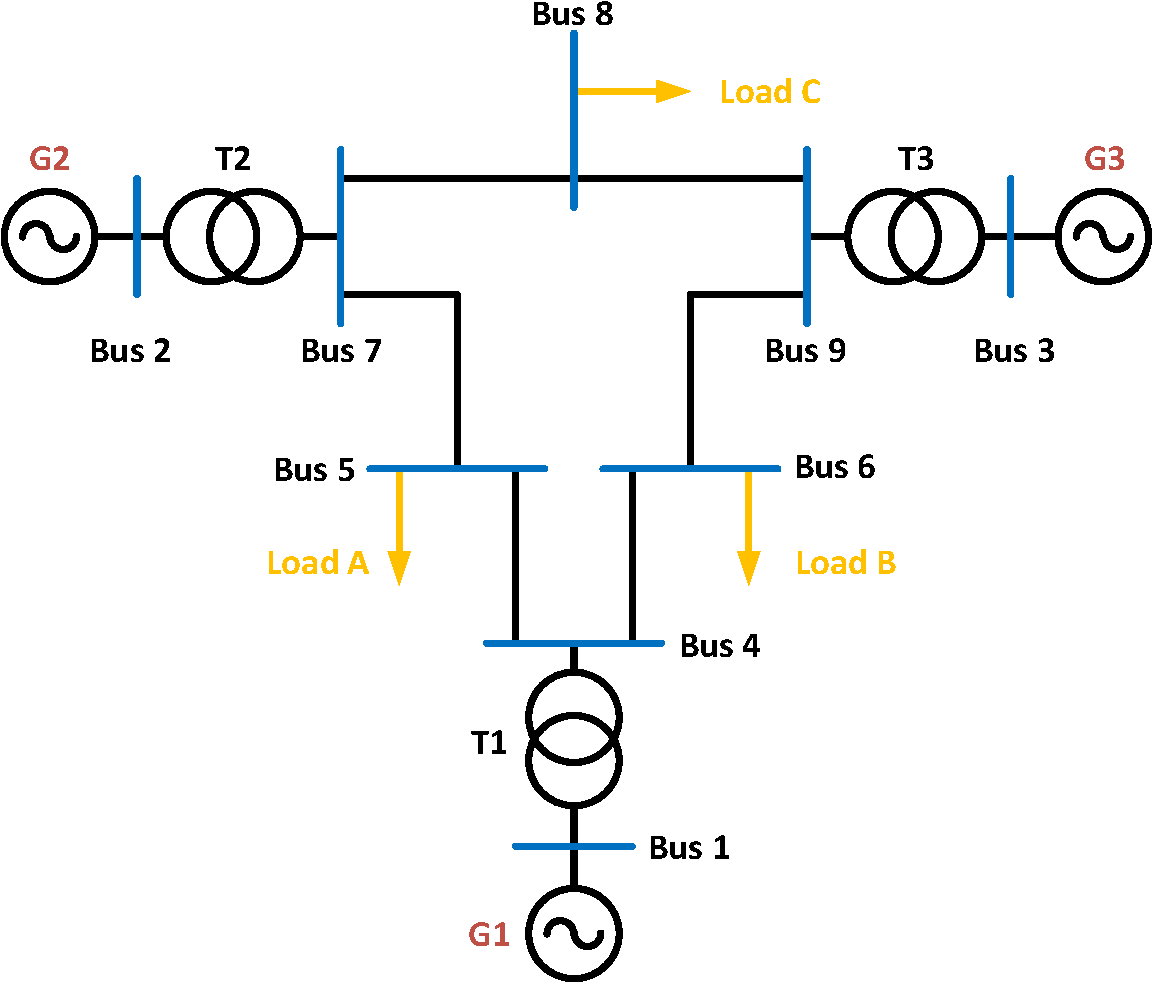
\includegraphics[width=.8\linewidth]{ieee_9_bus.pdf}
	\caption{P.M.Anderson Test Case}
	\label{ieee_9_bus}
\end{figure}
\begin{table}[h!]
	\centering
	\begin{tabular}{ccc}
		\hline
		\textbf{Generators} & \textbf{Active Power (MW)}  & \textbf{Reactive Power (MVAr)} \\ \hline
		Load A              & 125                      	  & 50				 \\
		Load B              & 90                          & 30                \\
		Load C              & 100                         & 35                \\ \hline
	\end{tabular}
	\caption{Load Properties of Test System}
	\label{loadproperties}
\end{table}
\subsection{Load Flow Analysis for Base Case}
Successful grid operation requires a load flow analysis in order to ensure that bus voltages are inside the allowed band and power flows are below the power carrying capabilities of the lines. Load flow results are tabulated in Table \ref{loadflow_case1}.
\begin{table}[h!]
	\centering
	\begin{tabular}{cclccccc}
		\hline
		Bus \# & Bus Type & \multicolumn{1}{c}{Voltage} & Angle & Pg    & Qg     & Pl  & Ql \\ \hline
		1      & SL       & \multicolumn{1}{c}{1.04}    & 0     & 71.65 & 27.05  & 0   & 0  \\
		2      & PV       & \multicolumn{1}{c}{1.025}   & 9.28  & 163   & 6.65   & 0   & 0  \\
		3      & PV       & \multicolumn{1}{c}{1.025}   & 4.66  & 85    & -10.86 & 0   & 0  \\
		4      & PQ       & 1.0258                      & -2.22 & 0     & 0      & 0   & 0  \\
		5      & PQ       & 0.9956                      & -3.99 & 0     & 0      & 125 & 50 \\
		6      & PQ       & 1.0126                      & -3.69 & 0     & 0      & 90  & 30 \\
		7      & PQ       & 1.0258                      & 3.72  & 0     & 0      & 0   & 0  \\
		8      & PQ       & 1.0159                      & 0.73  & 0     & 0      & 100 & 35 \\
		9      & PQ       & 1.0323                      & 1.97  & 0     & 0      & 0   & 0  \\ \hline
	\end{tabular}
	\caption{Load Flow Results in Base Case}
	\label{loadflow_case1}
\end{table}
\subsection{Base Case Frequency Response for Additional Load Connection}
It is obvious that power system networks experience high RoCoF when either high amount of generation trips or high amount of load connects to system. These two main event can be used in the simulation to create frequency disturbances. Since the simulation in Simulink environment slows down with the increasing amount of generators, the disturbances are created with load connections.\par
\begin{table}[h]
	\centering
	\begin{tabular}{ll}
		\hline
		Total System Load                      & 315 MW    \\
		Generator Droop Settings               & 5\%       \\
		Stored Kinetic Energy at Nominal Speed & 3.305 GWs \\
		Gen 1 Inertia Constant                 & 9.5515 s  \\
		Gen 2 Inertia Constant                 & 3.9216 s  \\
		Gen 3 Inertia Constant                 & 2.7665 s  \\ \hline
	\end{tabular}
	\caption{System Dynamical Properties}
	\label{systemdynamicaldata}
\end{table}
System dynamical properties are listed in Table \ref{systemdynamicaldata}. Power generation references are determined based on the load flow of powergui toolbox. Machine initialization toolbox is also used to initiate the state of generators in the system. However, the system does not start with the steady state. Still, system goes to steady state within a few seconds. Frequency of the network is disturbed with a load connection in the t=10 seconds in order to observe the frequency stability of the system. For 10\% load connection, a load of 31.5 MW is connected to system from Bus 6. Location of the additional load is depicted in Fig. \ref{ieee_9_bus_load}.\par
\begin{figure}[h]
	\centering
	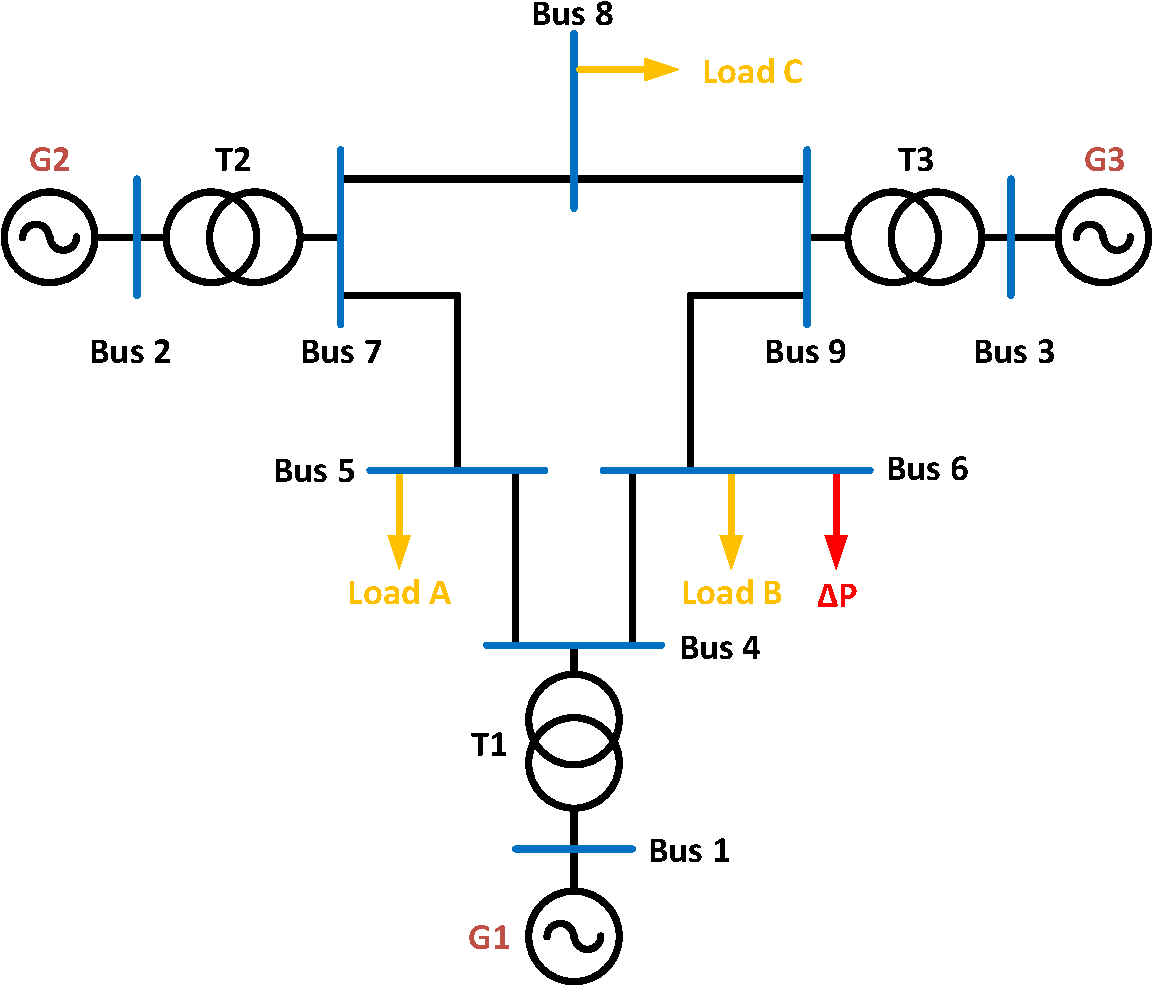
\includegraphics[width=.8\linewidth]{ieee_9_bus_load_position.pdf}
	\caption{Location of the Additional Load}
	\label{ieee_9_bus_load}
\end{figure}
According to the 10\% load connection to system, generator frequencies are shown in Fig. \ref{genfreqcase1}. As it can be seen from Fig. \ref{genfreqcase1}, rotor swings exists in the frequencies. However, the frequency of generator 1 is the most smooth one due to its huge inertia constant. Meanwhile, the generator 2 and generator 3 follow the frequency of generator 1 with higher rotor swings.\par
\begin{figure}[h!]
	\centering
	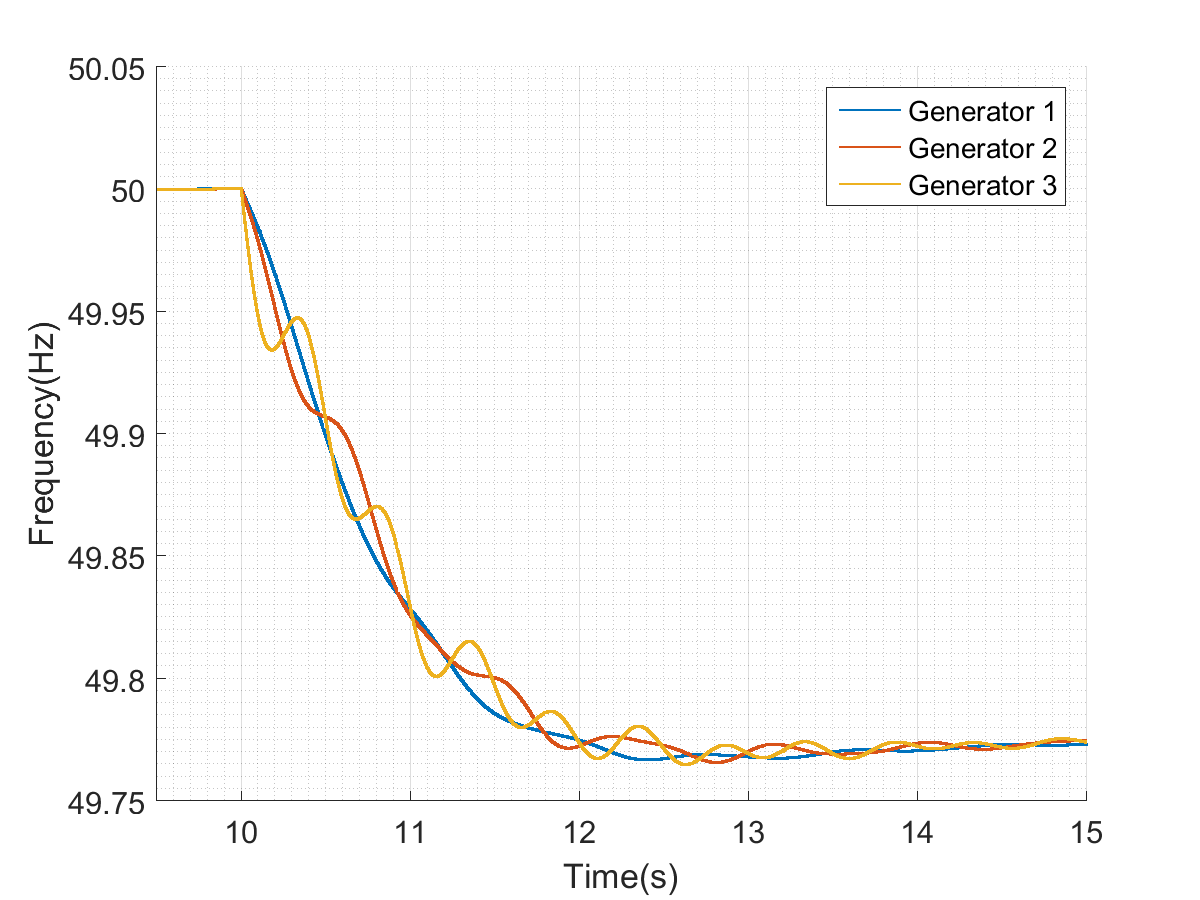
\includegraphics[width=.85\linewidth]{Case1_Generator_Freq.png}
	\caption{Generator Frequencies for 10\% Load Connection}
	\label{genfreqcase1}
\end{figure}
In the system, frequency of Bus 1 can be assumed as constant throughout the network since the system is small enough to assume a single frequency inside the network. This assumption can be verified by comparing the frequencies in Buses 1, 5 and 6. Fig. \ref{genfreqcase1_loadgen} shows the frequency of the generator 1 frequency as well as the load frequencies captured with Simulink PLL block. The only difference is the instant following the load connection. The sharp frequency decline delays the PLL loop to capture the frequency. 
\begin{figure}[h!]
	\centering
	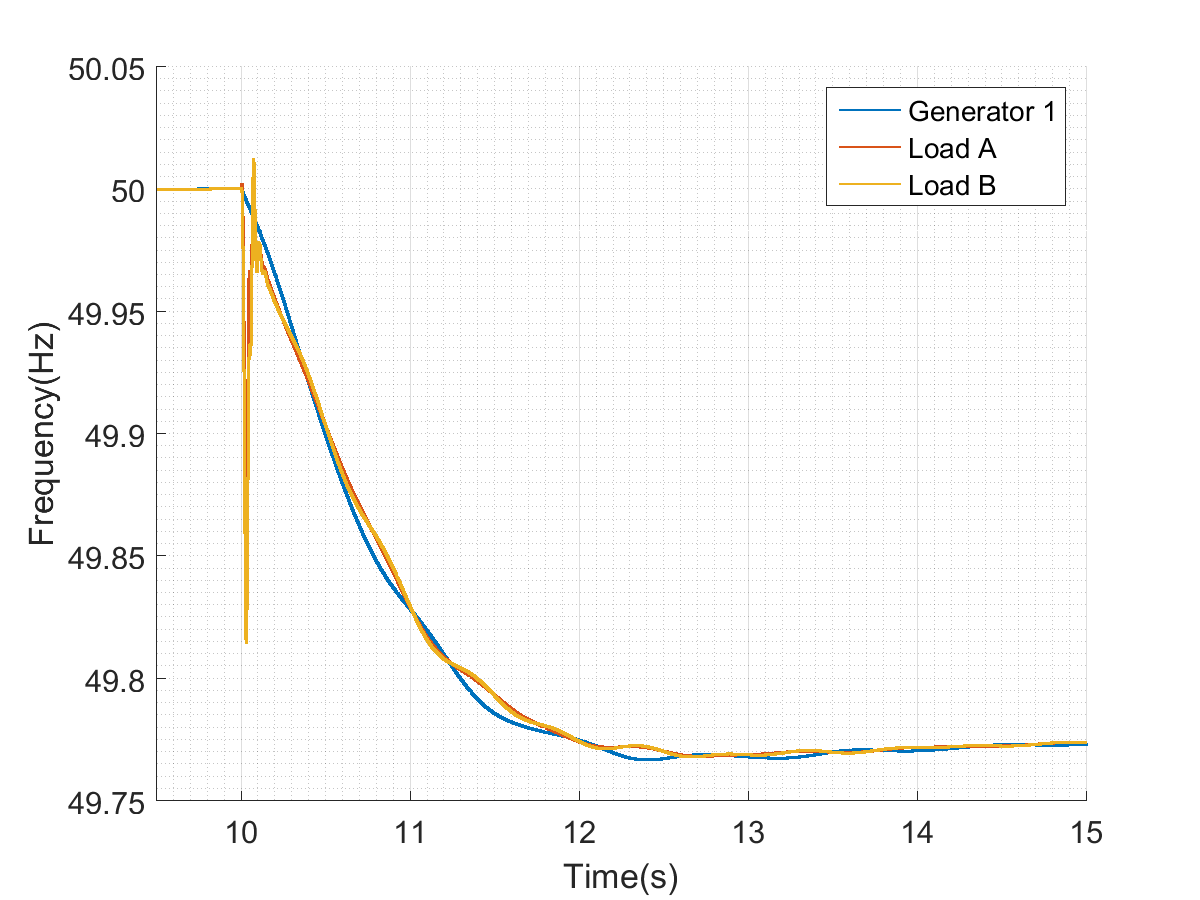
\includegraphics[width=.85\linewidth]{Case1_Load_Gen_Freq.png}
	\caption{Frequencies in Generator 1, Load A and Load B}
	\label{genfreqcase1_loadgen}
\end{figure}
\section{Modified Case}
\label{sec:kmodified}
In order to observe the effect of the renewable energy penetration to grid, the P.M. Anderson test case is modified such that a wind farm consists of 20 wind turbine is connected to network. Since the transmission network of the test case is under-utilized, the location of the wind farm has no effect on the frequency disturbance. Hence bus 5 is selected as the location for wind farm connection. Modified system is depicted in the Fig. \ref{ieee_9_bus_case2}. In this case, generator 2 and 3 are still assigned to same power generation references meanwhile generator 1 decreases its generation since it is the swing generator in the system. 
\begin{figure}[h!]
	\centering
	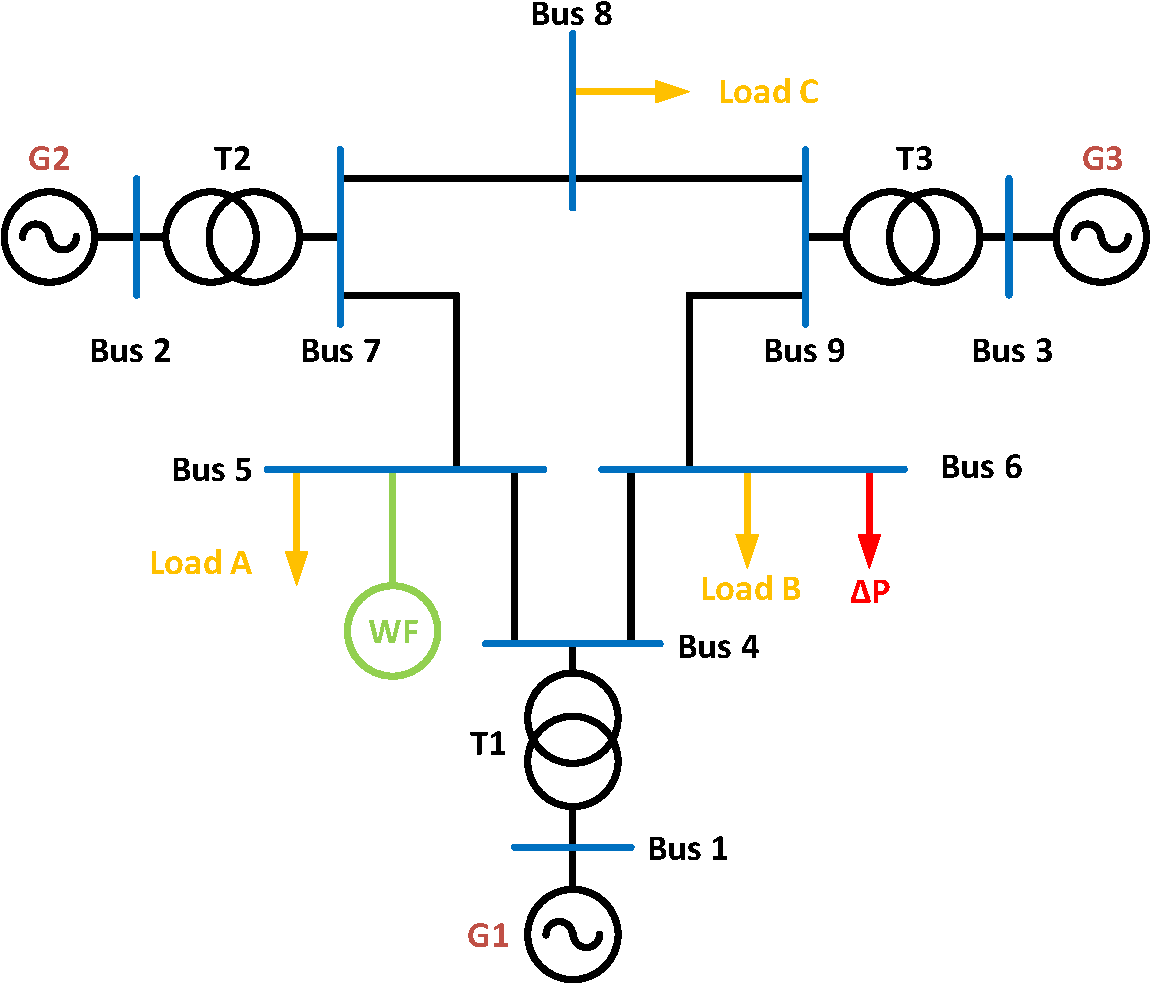
\includegraphics[width=.8\linewidth]{ieee_9_bus_modified.pdf}
	\caption{Modified System Single Line Diagram}
	\label{ieee_9_bus_case2}
\end{figure}
\subsection{Load Flow Analysis for Modified Case}
Load flow analysis for modified case is listed in Table \ref{loadflow_case2}. The power injected from Bus 1 is decreased as expected. This can also be seen from the phase angle between 1 and 4. Phase angle difference between these buses decreased from $2.22^{\circ}$ to $1.18^{\circ}$. Total power generation from active power from conventional generation units are also decreased. Therefore, the modified system resembles the base case with low power demand.
\begin{table}[h!]
	\centering
	\begin{tabular}{cclccccc}
		\hline
		Bus \# & Bus Type & \multicolumn{1}{c}{Voltage} & Angle & Pg    & Qg     & Pl  & Ql \\ \hline
		1      & SL       & \multicolumn{1}{c}{1.04}    & 0     & 38.06 & 25.07  & 0   & 0  \\
		2      & PV       & \multicolumn{1}{c}{1.025}   & 11.33 & 163   & 6.65   & 0   & 0  \\
		3      & PV       & \multicolumn{1}{c}{1.025}   & 6.32  & 85    & -10.86 & 0   & 0  \\
		4      & PQ       & 1.0263                      & -1.18 & 0     & 0      & 0   & 0  \\
		5      & PQ       & 0.9995                      & -1.54 & 0     & 0      & 125 & 50 \\
		6      & PQ       & 1.0128                      & -2.43 & 0     & 0      & 90  & 30 \\
		7      & PQ       & 1.0266                      & 5.77  & 0     & 0      & 0   & 0  \\
		8      & PQ       & 1.0164                      & 2.62  & 0     & 0      & 100 & 35 \\
		9      & PQ       & 1.0326                      & 3.62  & 0     & 0      & 0   & 0  \\ \hline
	\end{tabular}
	\caption{Load Flow Results for Modified Case}
	\label{loadflow_case2}
\end{table}
\subsection{Modified Case Frequency Response for Additional Load Connection}
The modified base is very similar to the Base Case except for a wind farm located in Bus 5. The renewable energy system in this case can be considered as a negative load. Therefore, base case with decreased load is under discussion in this subsection. The same amount of load is taken into operation at Bus 6 and the frequency response of the modified system is shown in Fig. \ref{Case1_2_freq}. \par
\begin{figure}[h!]
	\centering
	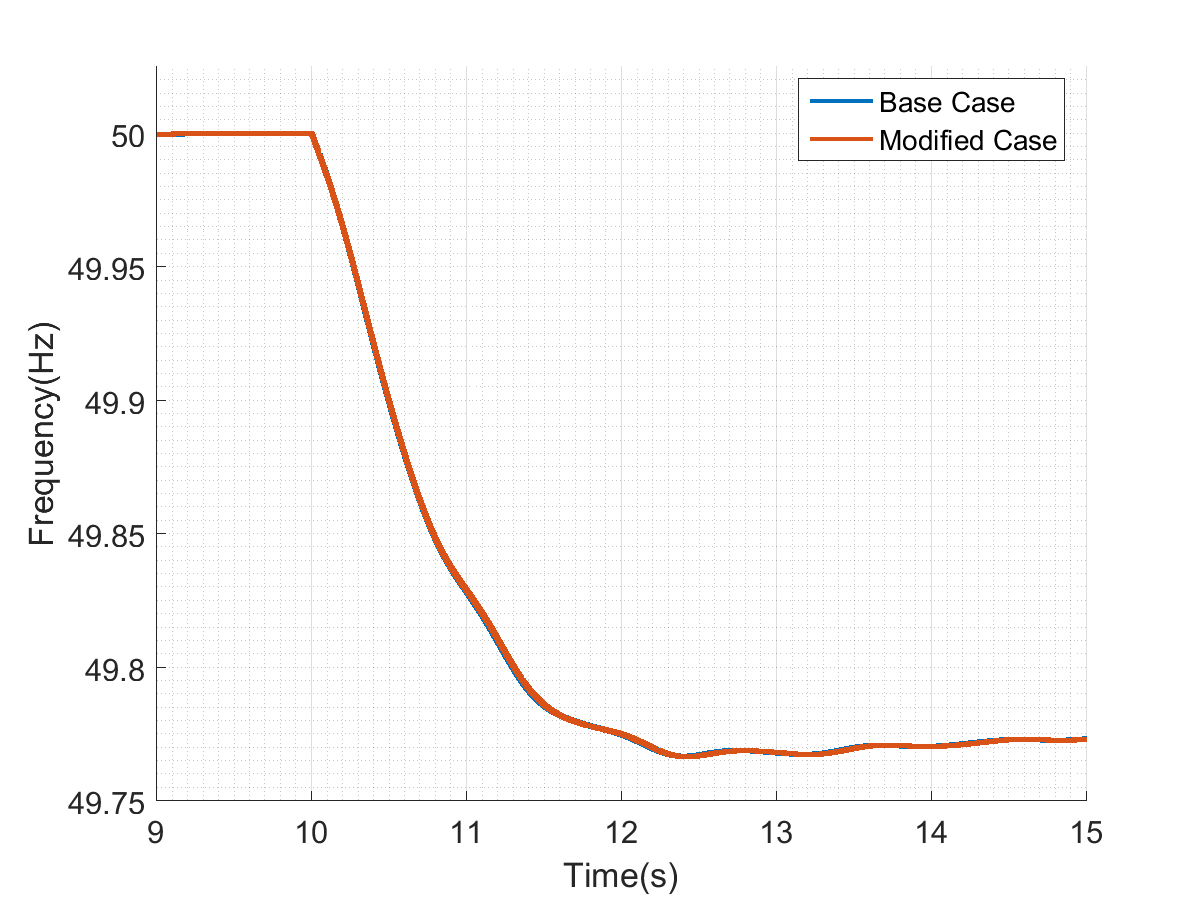
\includegraphics[width=.85\linewidth]{Case1_2.png}
	\caption{Comparison of Base Case and Modified Case Frequencies}
	\label{Case1_2_freq}
\end{figure}
Almost the same frequency response is observed in the system. The reason is that both systems have the same amount of stored kinetic energy. Another reason is that there is no congestion in the system due to under-utilized of transmission network. The same frequency response can also be observed in the rate of change of frequencies in Fig. \ref{Case1_2_rocof}. Almost the same RoCoF values are observed in the system. This concludes that renewable energy penetration does not change frequency response of the system if the only change in the system is the inclusion of renewable energy system. In other words, renewable energy systems does not affect the frequency response of the grid unless the system is replaced with a conventional generation unit. Note that the renewable energy systems are intermittent energy sources. However, in this study,the source of the renewable energy system is assumed as constant. Therefore, the reason of frequency disturbance is load connection rather than the change in active power output of renewable systems.
\begin{figure}[h!]
	\centering
	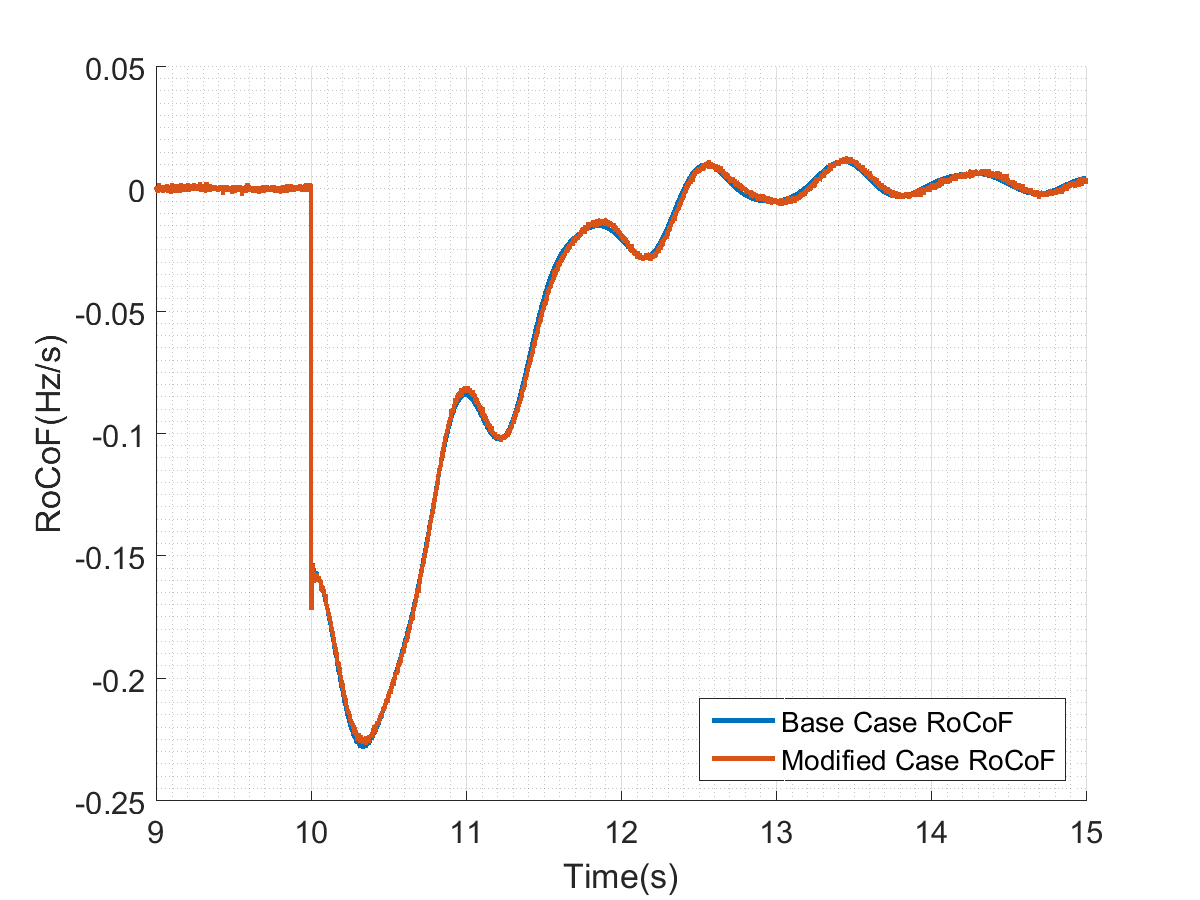
\includegraphics[width=.85\linewidth]{Case1_2_rocof.png}
	\caption{Comparison of Base Case and Modified Case Frequencies}
	\label{Case1_2_rocof}
\end{figure}
\section{Decommissioned Case}
\label{sec:kdecommissioned}
As seen in the Modified Case, the frequency response of the system does not change with renewable energy inclusion. However, it is inevitable that renewable energy systems will replace the conventional units in future. In this case, the smallest generator, generator 3, will be decommissioned due to economical concerns. The decommissioned case diagram is shown in Fig. \ref{decommissioned_case}.\par
\begin{figure}[h!]
	\centering
	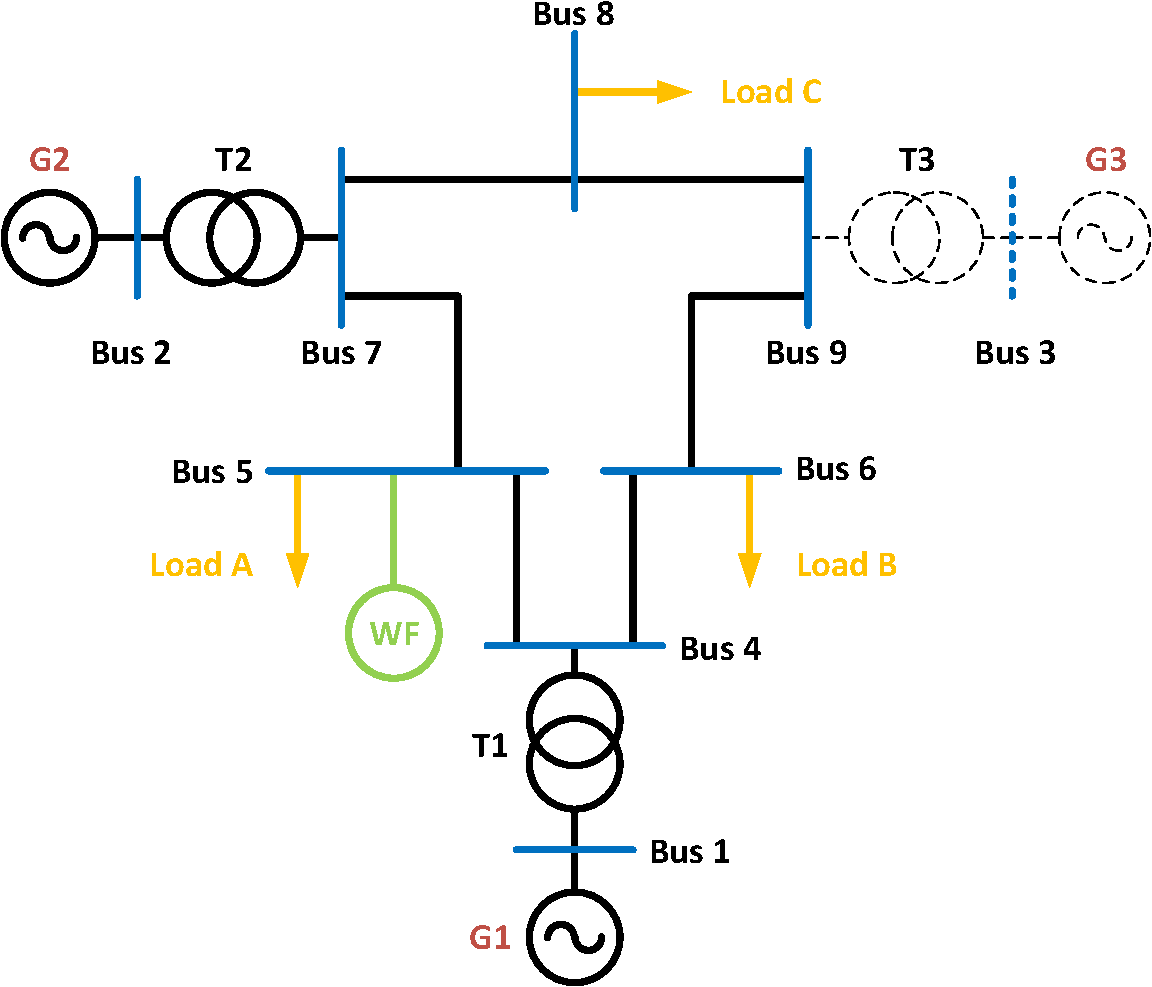
\includegraphics[width=.8\linewidth]{ieee_9_bus_decommissioned.pdf}
	\caption{Decommissioned Case Sinle Line Diagram}
	\label{decommissioned_case}
\end{figure}
Since the generator 3 is out of service, the stored kinetic energy is decreased in the system. Decommissioned system dynamical properties are updated and given in Table \ref{systemdynamicaldatacase3}. Higher RoCoF value and lower frequency nadir are expected with the same additional load since the system dynamical properties are deteriorated with the removal of generator 3.
\begin{table}[h]
	\centering
	\begin{tabular}{ll}
		\hline
		Total System Load                      & 315 MW    \\
		Generator Droop Settings               & 5\%       \\
		Stored Kinetic Energy at Nominal Speed & 3.004 GWs \\
		Gen 1 Inertia Constant                 & 9.5515 s  \\
		Gen 2 Inertia Constant                 & 3.9216 s  \\
		\hline
	\end{tabular}
	\caption{System Dynamical Properties}
	\label{systemdynamicaldatacase3}
\end{table}
\subsection{Load Flow Analysis for Decommissioned Case}
Since the generator 3 is out of service, generator 1 loading will be increased. Load flow analysis for decommissioned case is given in Table \ref{loadflow_case3}.
\begin{table}[h!]
	\centering
	\begin{tabular}{cclccccc}
		\hline
		Bus \# & Bus Type & \multicolumn{1}{c}{Voltage} & Angle & Pg    & Qg     & Pl  & Ql \\ \hline
		1      & SL       & \multicolumn{1}{c}{1.04}    & 0     & 121.76& 16.26  & 0   & 0  \\
		2      & PV       & \multicolumn{1}{c}{1.025}   & 4.18  & 163   & 0.65   & 0   & 0  \\
		4      & PQ       & 1.0332                      & -3.74 & 0     & 0      & 0   & 0  \\
		5      & PQ       & 1.0083                      & -5.63 & 0     & 0      & 125 & 50 \\
		6      & PQ       & 1.0224                      & -7.65 & 0     & 0      & 90  & 30 \\
		7      & PQ       & 1.0294                      & -1.36 & 0     & 0      & 0   & 0  \\
		8      & PQ       & 1.0207                      & -5.82 & 0     & 0      & 100 & 35 \\
 \hline
	\end{tabular}
	\caption{Load Flow Results for Decommissioned Case}
	\label{loadflow_case3}
\end{table}
\subsection{Decommissioned Case Frequency Response for Additional Load Connection}
Decommissioned system is also subjected to the same frequency disturbance which is the additional load connection from Bus 6. System frequency response is observed and compared to Base Case and Modified Case in Fig. \ref{Case1_2_3_freq}. The frequency response of the system gets worse with the generator 3 decommissioned. It results that the frequency nadir is decrease from 49.77Hz to 49.65Hz due to the decrease in the stored kinetic energy in the system. The deteriorated frequency response can also be seen from the comparison of RoCoFs that is given in Fig. \ref{Case1_2_3_rocof}. 
\begin{figure}[h]
	\centering
	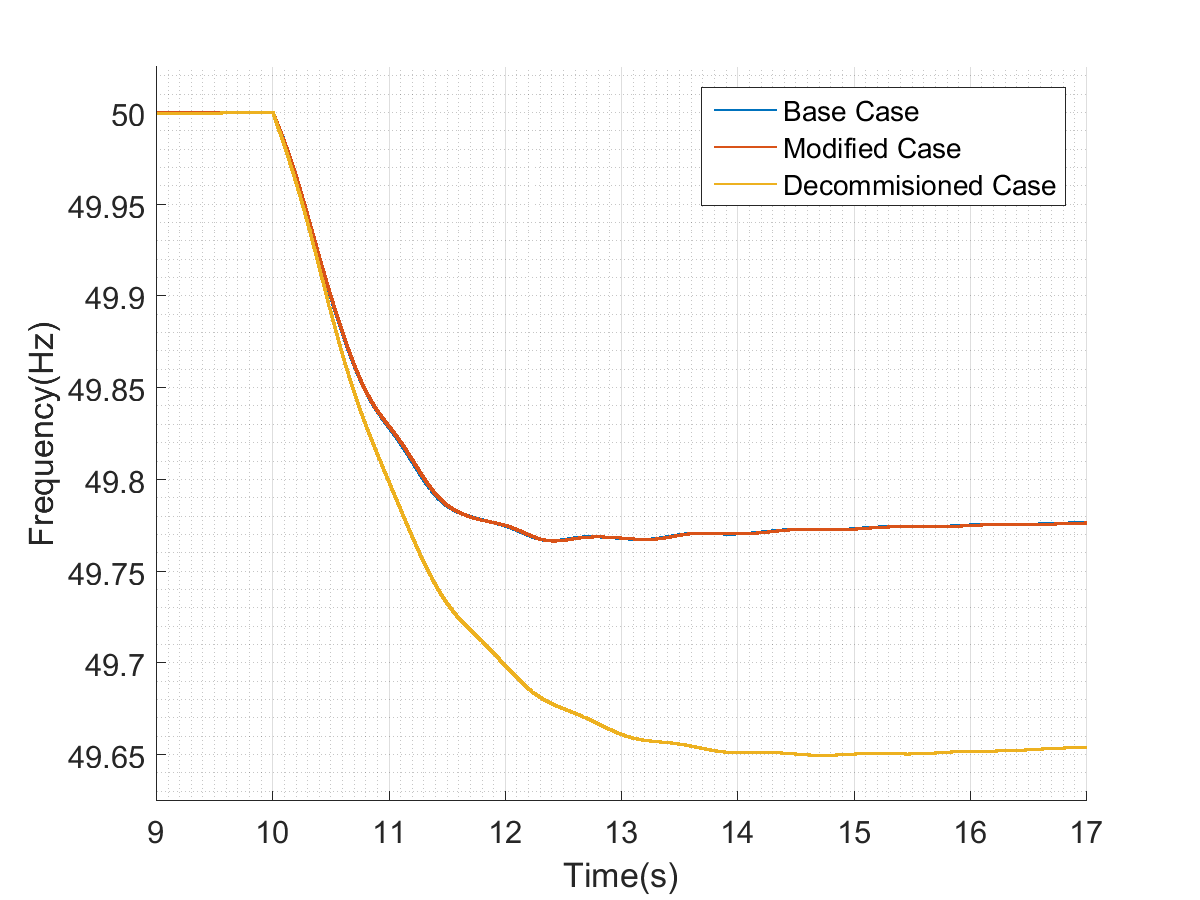
\includegraphics[width=.85\linewidth]{Case1_2_3_freq.png}
	\caption{Comparison of Base Case,Modified Case and Decommissioned Case Frequency Responses}
	\label{Case1_2_3_freq}
\end{figure}
\begin{figure}[h]
	\centering
	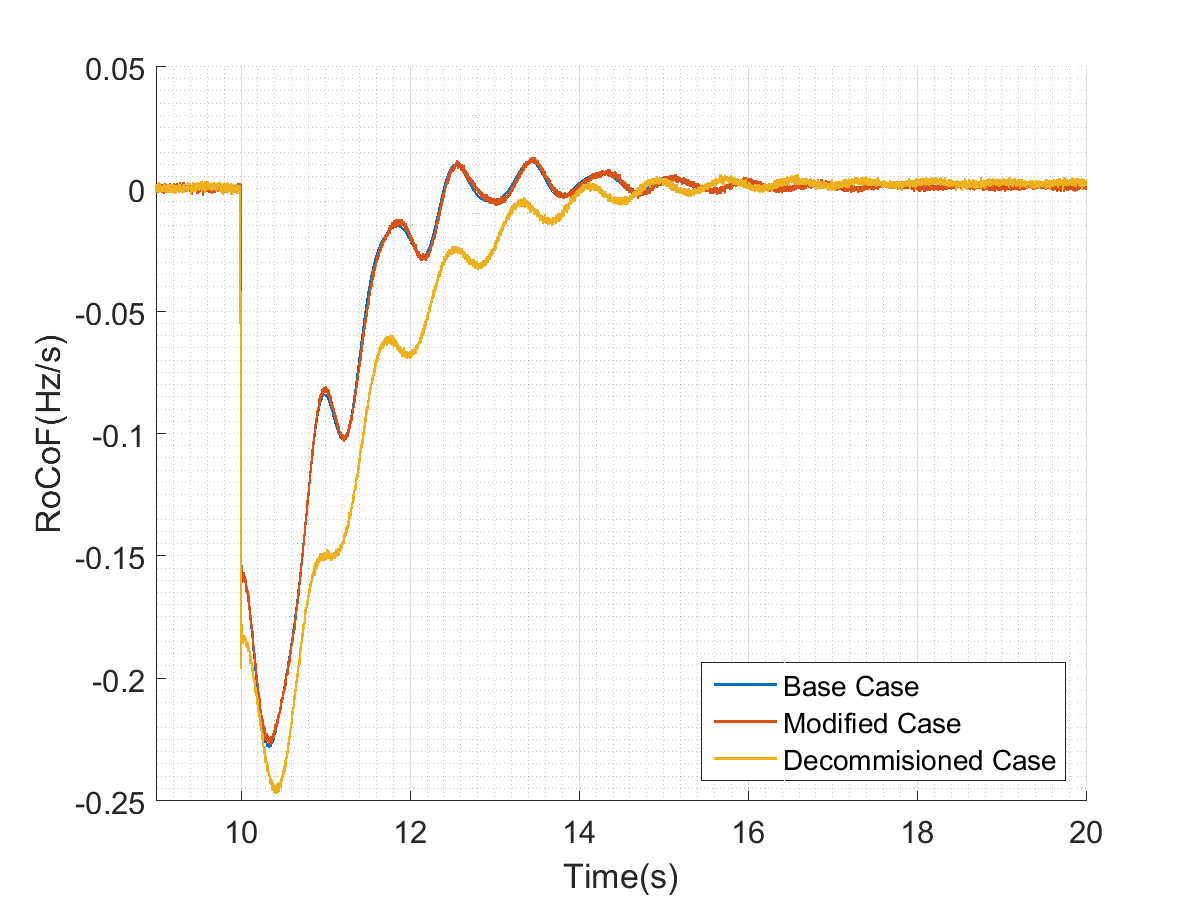
\includegraphics[width=.85\linewidth]{Case1_2_3_rocof.png}
	\caption{Comparison of Base Case,Modified Case and Decommissioned Case RoCoFs}
	\label{Case1_2_3_rocof}
\end{figure}
\section{Modified Case with Synthetic Inertia}
The frequency response of the modified system is investigated in Section \ref{sec:kmodified} and the system frequency was almost the same with test system base case. However, the response of the system can be improved by provision of synthetic inertia. The wind turbines in the system is equipped with synthetic inertia that emulates inertia constants of 5s, 10s and 15s. The system response with inertial support provision is given in the Fig. \ref{Case4_freq}.\par
\begin{figure}[h!]
	\centering
	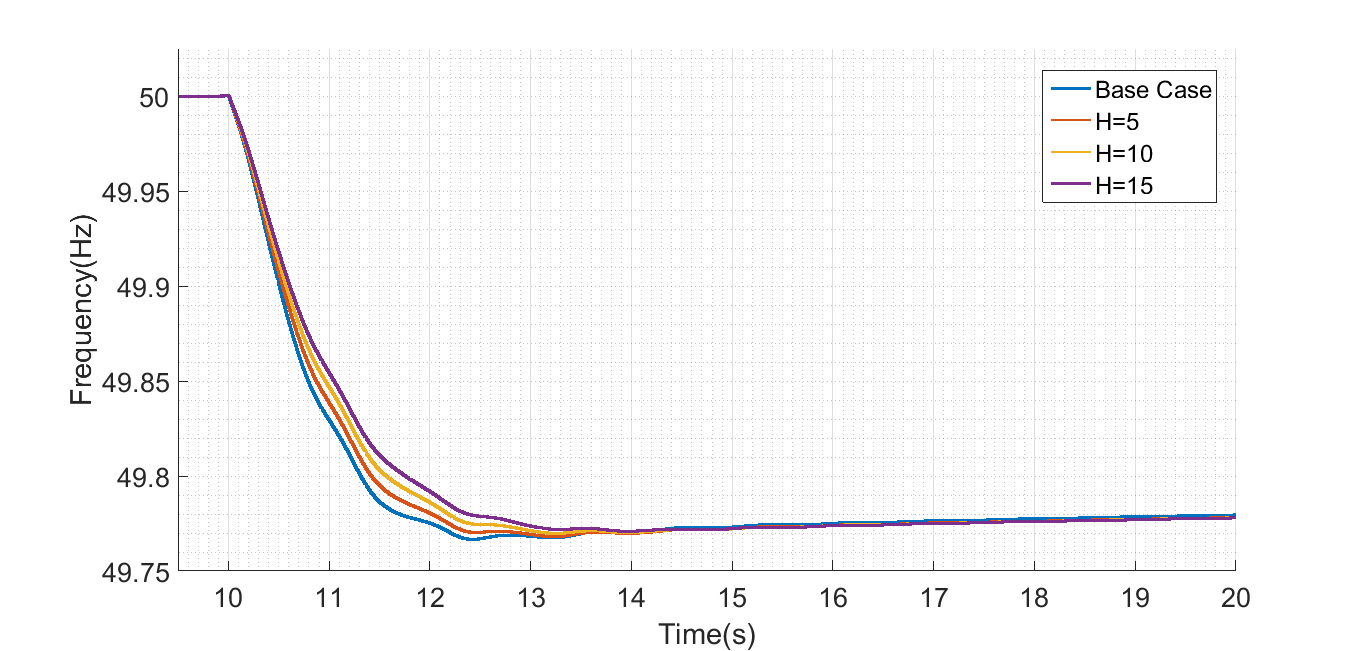
\includegraphics[width=.9\linewidth]{case4_frequencies.png}
	\caption{Emulation of the Different Inertia Constants for the Modified Case}
	\label{Case4_freq}
\end{figure}
Since the modified case frequency response is almost the same with the base case, the synthetic inertia implementation is improved the system frequency response. In other words, the wind turbines are integrated to the system by emulating the synchronous generator behaviour. It is to note that huge amount of kinetic energy exists in the wind turbine systems. That stored energy can be utilized with the synthetic inertia method in order to improve frequency dynamics of the system.\par
Emulation of synchronous generator behaviour is basically increasing the amount of active power depending on the RoCoF of the grid and the inertia constant to be emulated. Since the higher inertia constant requires higher active power increase, the inertia constants of 10s and 15s result in better frequency dynamics. The frequency nadir of the base case is slightly increased. The effect of the synthetic inertia provision can also be observed in the system RoCoF values that is given in Fig. \ref{Case4_rocof}.\par
\begin{figure}[h]
	\centering
	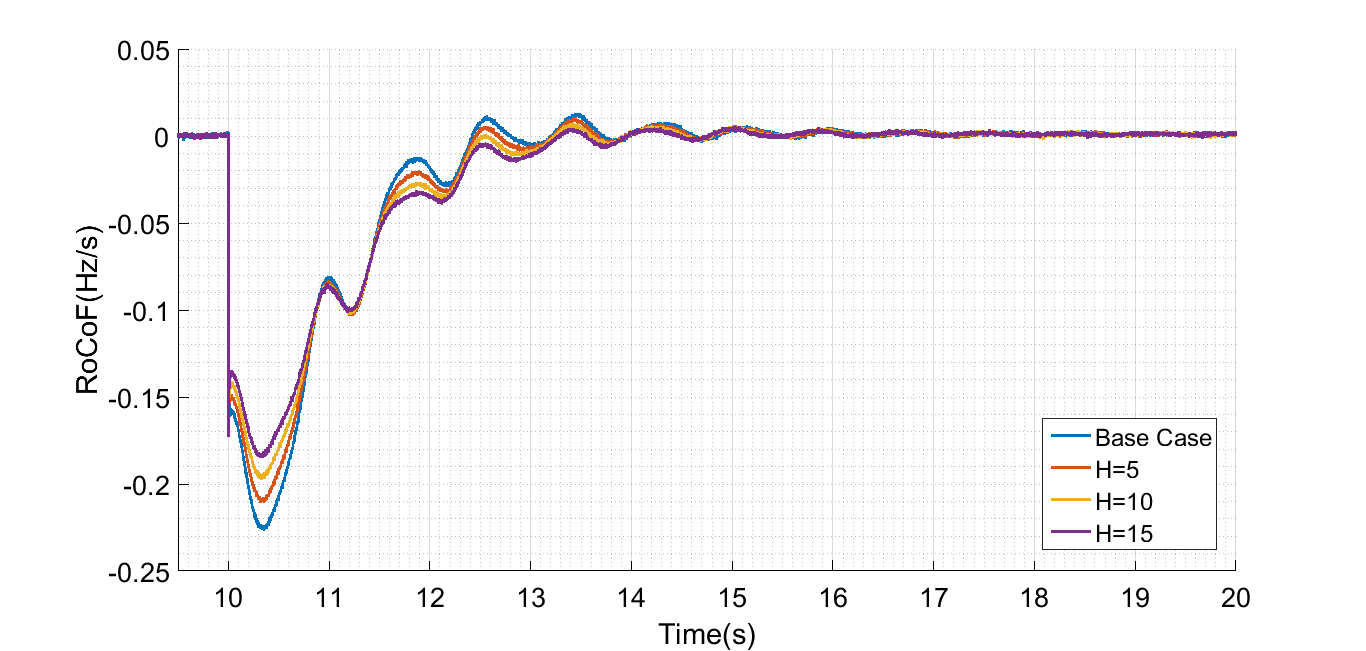
\includegraphics[width=1\linewidth]{case4_rocof.png}
	\caption{RoCoF of the Different Inertia Constants for the Modified Case}
	\label{Case4_rocof}
\end{figure}
It is obvious that the base case experience the highest RoCoF in the very first second of the frequency disturbance. While the remaining cases is subjected to lower RoCoF at first, the base case RoCoF is the lowest following seconds. The reason is that the base case active power contribution in the first second is much higher than others. Hence, the case subjected to severe conditions react higher and faster resulting quick restoration of the system. Another observation is that all cases converges to the same steady state frequency due to the fact that inertial support affects the transient rather than the steady state values. The steady state frequency is dependent on the capacity of conventional synchronous generators and their droop constants. This is why the decommissioned case steady state frequency is lower than that of modified case.
\section{Decommissioned Case with Synthetic Inertia}
Decommissioned case frequency response for 10\% additional load connection is studied in the Section \ref{sec:kdecommissioned}. System frequency experiences high RoCoF and lower steady state frequency because of the removal of the generator 3. In this section, synthetic inertia method  is implemented on the decommissioned case wind farm with different inertia constants. The resultant frequency responses are shown in the Fig. \ref{Case5_freq}. As in the case of modified case, base case frequency response experiences steepest decline in the frequency meanwhile the higher inertia constant synthetic inertia implementations have smoother frequency decrease.\par
\begin{figure}[h]
	\centering
	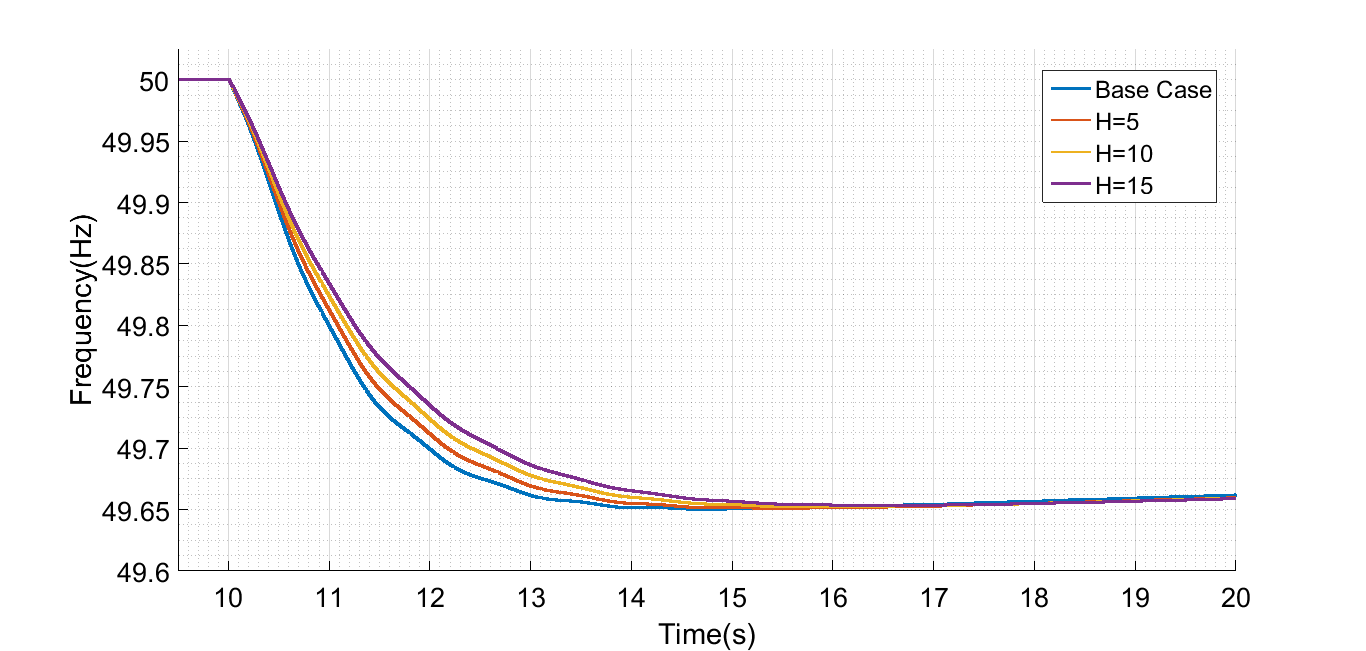
\includegraphics[width=0.9\linewidth]{case5_frequency.png}
	\caption{RoCoF of the Different Inertia Constants for the Decommissioned Case}
	\label{Case5_freq}
\end{figure}
The active power of the wind turbine for the different inertia constants is given in Fig. \ref{Case5_power}. It should be noted that the active power of the wind turbine is proportional with the RoCoF that is also given in Fig. \ref{Case5_rocof}. Note that 15s inertia constant is also emulated. It is stated that conventional generator inertia constants lie between 2-9s \cite{Kundur}. Nonetheless, synchronous generators have constant kinetic energy in the nominal frequency. However, the kinetic energy stored in the turbine inertia fluctuates with the generator speed. Moreover, wind turbine is able to emulate different inertia constant as soon as it has the capacity to increase its power. Even with the inertia constant of 15s, the wind turbine is far away from its maximum allowable power. Therefore, higher inertia constants can also be tested in the expense of longer speed recovery process whose resultant decreased power might also affect the RoCoF further. 
\begin{figure}[h]
	\centering
	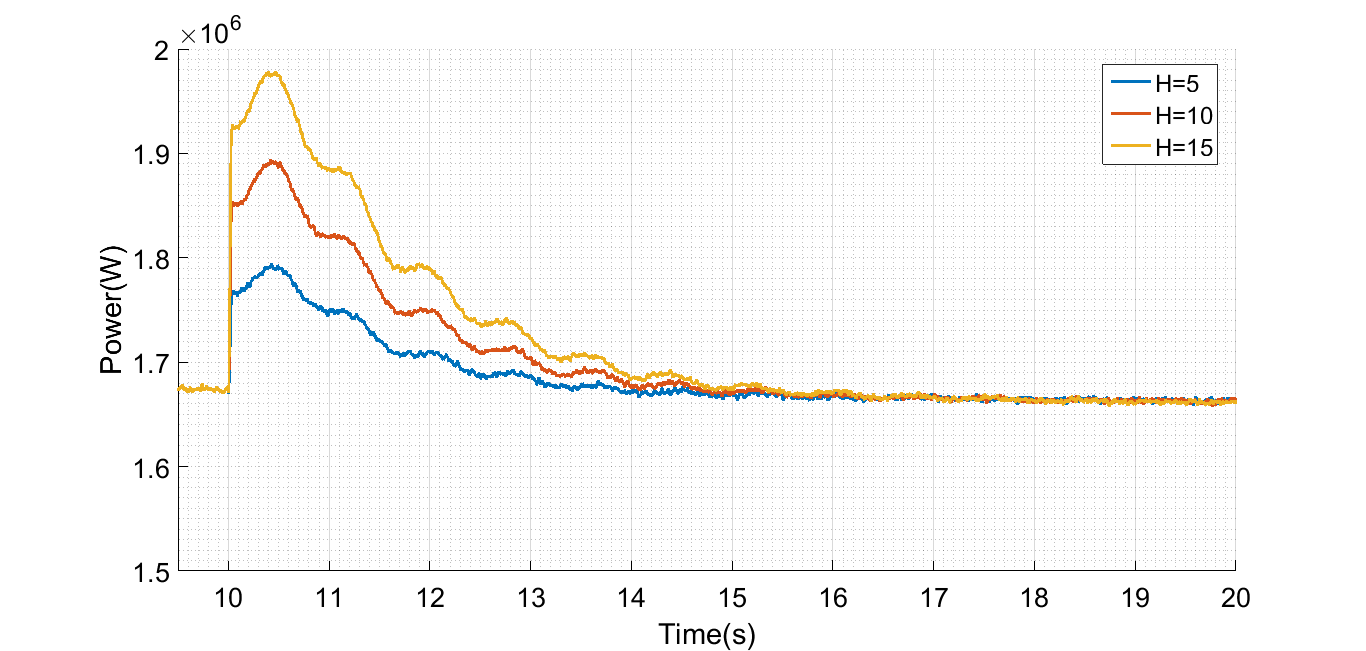
\includegraphics[width=0.9\linewidth]{case5_powers.png}
	\caption{Wind Turbine Active Power for the Different Inertia Constants in the Decommissioned Case}
	\label{Case5_power}
\end{figure}
\begin{figure}[h!]
	\centering
	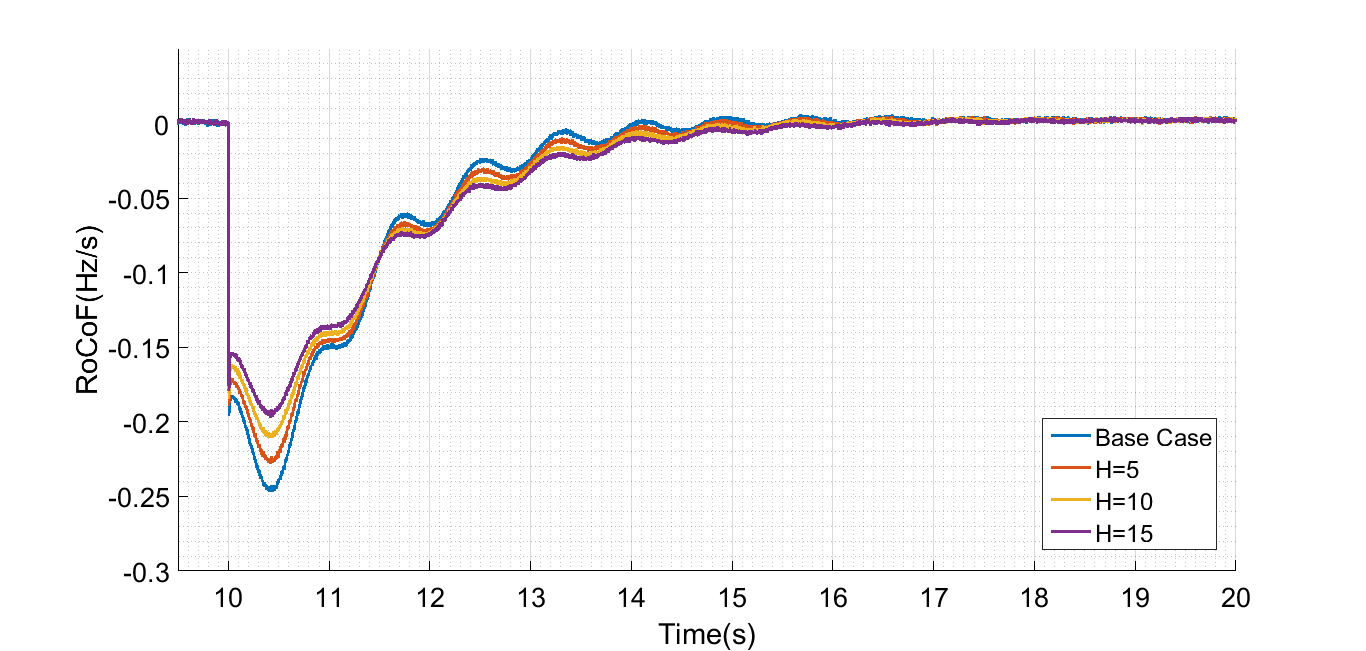
\includegraphics[width=0.9\linewidth]{case5_rocof.png}
	\caption{Wind Turbine Active Power for the Different Inertia Constants in the Decommissioned Case}
	\label{Case5_rocof}
\end{figure}
\section{Comparison of the Synthetic Inertia and Fast Inertial Support}
In the Chapter \ref{chp:4}, it is stated that the wind turbines have more than sufficient capacity in order to increase its active power. The fast inertial support concept is studied with different increase rates. The exaggerated inertial supports are studied to observe the turbine internal dynamics. In this section, the fast inertial support will be compared with the synthetic inertia. In other words, increasing active power by a defined percentage will be compared to a rise in the active power proportional to RoCoF. For this reason, the same frequency disturbance is tested on the base case decommissioned case, the case where inertia constant of 10s is emulated and also the one with fast inertial support with 5\% increased power by 5 seconds. Fig. \ref{Comp_power} shows the variation of the active power. In order to increase the effectiveness of the fast inertial support, it is activated with a delay of 0.25s. In this interval, the synchronous generators take action for the upcoming disturbance. It should be underlined that the active power of the inertia emulated case is increased proportional to the RoCoF. Therefore, it declines as the RoCoF declines. Therefore, in the other half of the support time, it is below of the fast inertial support case. This phenomena can be clearly observed in the frequency response.\par
\begin{figure}[h]
	\centering
	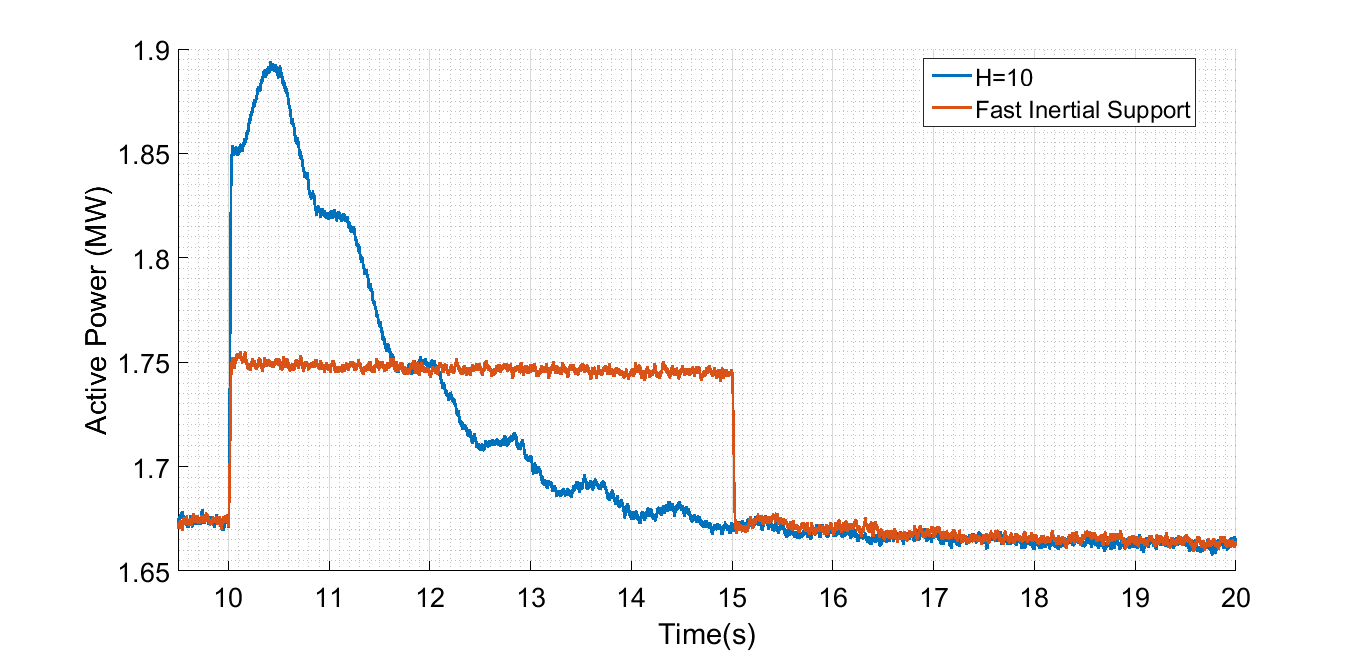
\includegraphics[width=0.9\linewidth]{comparison_power.png}
	\caption{Comparison of the Frequency Responses for the Base, Fast Inertial Support and Synthetic Inertia Cases}
	\label{Comp_power}
\end{figure}
The frequency response of these three cases is shown in Fig. \ref{Comp_freq}. It is obvious that the base case frequency response has the poorest transient frequency. Besides, the synthetic inertia implemented case has the best transient behaviour for the very first seconds. Nonetheless, the fast inertial support case first converges to higher steady state frequency until the end of the support period. However, as soon as the support ends, the sharp decrease in the active power results a second dip in the frequency. In contrary, the synthetic inertia case active power is decreased down to lower values as the RoCoF is positive. Than means that the recovery process is already started inside the support. Hence, the secondary dip is not observed in this case. 
\begin{figure}[h!]
	\centering
	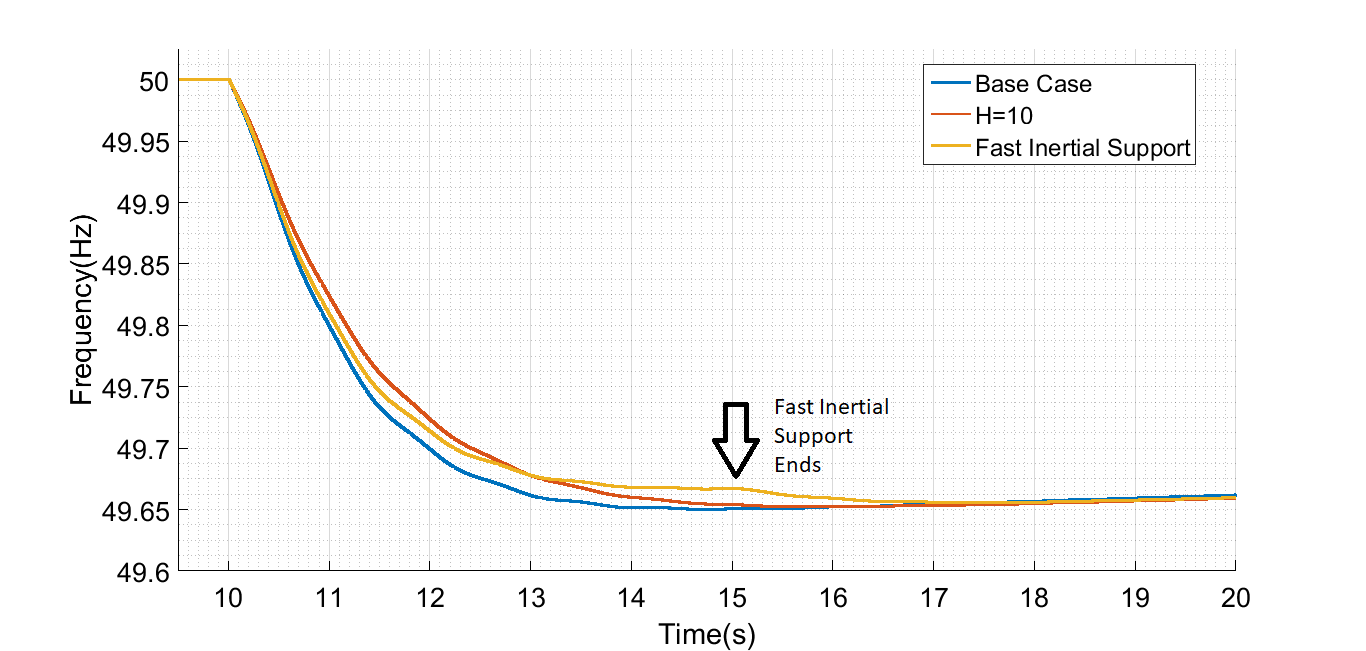
\includegraphics[width=0.9\linewidth]{comparison_freq.png}
	\caption{Comparison of the Active Power Increase in Fast Inertial Support Case and Synthetic Inertia Case}
	\label{Comp_freq}
\end{figure}